\section{Results}

\begin{figure*}[!t]
\centering
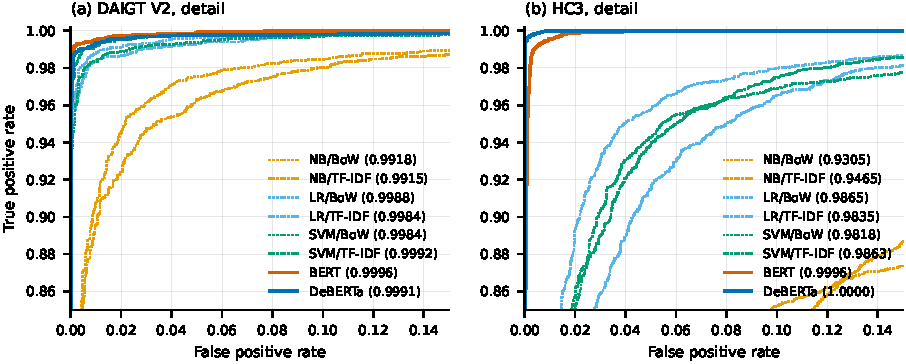
\includegraphics[width=\textwidth]{figures/fig_roc_zoom.pdf}
\caption{ROC curves for all eight model configurations, restricted to the low-false-positive region where the models actually differ. Areas under the full curve are given in the legend. On DAIGT V2 (a) every configuration converges toward the corner and the classical models are close behind the transformers. On HC3 (b) the two transformers separate sharply from all six classical configurations. Colours are colourblind-safe and each series carries a distinct dash pattern, so the ordering survives greyscale reproduction.}
\label{fig:roc}
\end{figure*}

\begin{figure*}[!t]
\centering
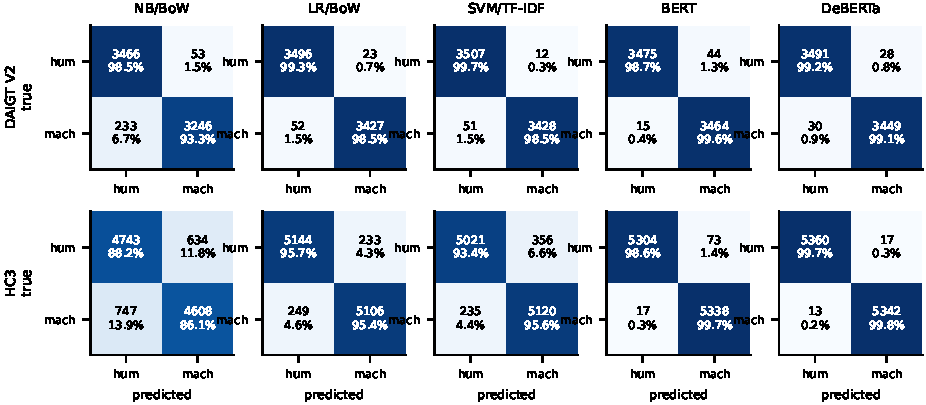
\includegraphics[width=\textwidth]{figures/fig_confusion.pdf}
\caption{Confusion matrices for the best configuration of each model family, both datasets, as counts and row-normalised percentages. Naive Bayes on HC3 is the only cell with substantial error in both directions, and every other cell concentrates its error on one side.}
\label{fig:confusion}
\end{figure*}

\begin{table}[!t]
\centering
\caption{All model configurations, both datasets, deployed checkpoints only. Error rate is reported beside F1 because F1 differences compress at this ceiling. Macro F1 equals weighted F1 to four decimals in every row, so no result is produced by class skew.}
\label{tab:allmodels}
\small
\begin{tabular}{@{}llcccc@{}}
\toprule
& & \multicolumn{2}{c}{DAIGT V2} & \multicolumn{2}{c}{HC3} \\
\cmidrule(lr){3-4}\cmidrule(lr){5-6}
Model & Rep. & F1 & err\,\% & F1 & err\,\% \\
\midrule
Naive Bayes & BoW & 0.9591 & 4.09 & 0.8713 & 12.87 \\
Naive Bayes & TF-IDF & 0.9577 & 4.23 & 0.8670 & 13.28 \\
Logistic Reg. & BoW & 0.9893 & 1.07 & \textbf{0.9551} & 4.49 \\
Logistic Reg. & TF-IDF & 0.9857 & 1.43 & 0.9365 & 6.35 \\
SVM & BoW & 0.9870 & 1.30 & 0.9475 & 5.25 \\
SVM & TF-IDF & \textbf{0.9910} & 0.90 & 0.9449 & 5.51 \\
BERT & raw & 0.9916 & 0.84 & 0.9916 & 0.84 \\
DeBERTa & raw & \textbf{0.9917} & 0.83 & \textbf{0.9972} & 0.28 \\
\bottomrule
\end{tabular}
\end{table}

\subsection{A classical model matches a transformer on DAIGT V2 but not on HC3}

Table~\ref{tab:allmodels} reports every model configuration on both datasets, and Fig.~\ref{fig:roc} gives the corresponding ROC curves and areas. The two benchmarks behave differently in a way no single headline number reveals. On DAIGT V2 the best classical configuration, an SVM over TF-IDF at 0.9910 F1, sits 0.0007 below the best transformer at 0.9917, a difference well inside the 0.0036 seed range we measure for this family of runs. On HC3 the same comparison is 0.9551 against 0.9972, an error-rate ratio of 16 to one. Whatever the transformers contribute on HC3, they contribute almost none of it on DAIGT V2.

Ranking by area does not reproduce ranking by F1. On DAIGT V2, BERT attains the higher area, 0.9996 against 0.9991, while DeBERTa attains the higher F1. We report both rather than the more favourable one.

\subsection{On HC3, orthography alone matches content alone}

\begin{table}[!t]
\centering
\caption{Surface-content decomposition. Surface-only uses 47 orthographic features and never reads a word. Content-only strips punctuation, casing and non-ASCII before vectorising. The transformer is a reference point, not a matched arm.}
\label{tab:decomp}
\small
\begin{tabular}{@{}lcccc@{}}
\toprule
& \multicolumn{2}{c}{DAIGT V2} & \multicolumn{2}{c}{HC3} \\
\cmidrule(lr){2-3}\cmidrule(lr){4-5}
Arm & F1 & err\,\% & F1 & err\,\% \\
\midrule
surface-only & 0.9214 & 7.86 & \textbf{0.9680} & \textbf{3.20} \\
content-only & \textbf{0.9901} & \textbf{0.99} & 0.9674 & 3.26 \\
full transformer & 0.9917 & 0.83 & 0.9972 & 0.28 \\
\bottomrule
\end{tabular}
\end{table}

\begin{figure}[!t]
\centering
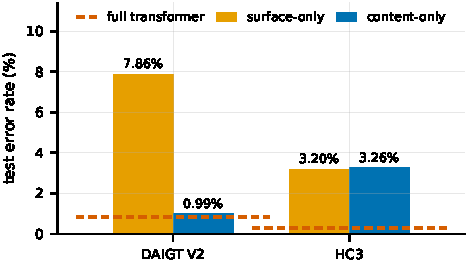
\includegraphics[width=\columnwidth]{figures/fig_decomposition.pdf}
\caption{Test error for the surface-only and content-only arms, with the best full transformer marked. On HC3 the two arms coincide. On DAIGT V2 content is stronger by a factor of 7.9 in error.}
\label{fig:decomp}
\end{figure}

Table~\ref{tab:decomp} and Fig.~\ref{fig:decomp} give the decomposition. On HC3 the two arms are indistinguishable, 3.20\% error from orthography against 3.26\% from content. Forty-seven features that never read a word do as well as a bag-of-words model over the whole vocabulary. On DAIGT V2 the same two arms separate by a factor of 7.9 in error, 7.86\% against 0.99\%, with content the stronger by a wide margin.

Two qualifications belong with this result rather than after it. First, surface form is informative on both benchmarks. DAIGT V2's surface-only arm reaches 0.9214 F1, far above chance, so the finding is not that one dataset is clean and the other is not. It is that only on HC3 does surface form rise to parity with content. Second, an earlier version of this analysis used a single hand-chosen threshold on one whitespace feature and concluded that DAIGT V2 was separable at chance. That conclusion was an artefact of the instrument, not a property of the dataset, and a fitted multi-feature model overturns it. We report the fitted result and retract the threshold one.

The content-only arm also bounds what the transformers add. On DAIGT V2 content-only reaches 0.9901 against the transformer's 0.9917, a difference inside the seed range, so the transformer adds nothing measurable over a bag-of-words model on surface-normalised text. On HC3 the transformer improves on either single arm by roughly 0.03 F1, consistent with combining information that neither arm holds alone.

\subsection{A model that cannot represent the cue reaches 0.9916 regardless}

The most-discussed HC3 artefact is a space preceding punctuation in human answers~\cite{Tian2023multiscale}, present in our copy at 10.745 occurrences per human document against 0.013 per machine document. It is natural to assume detectors exploit it. Tokenisation makes that assumption testable rather than rhetorical.

BERT's WordPiece tokeniser splits on punctuation irrespective of adjacent whitespace. For the pair \texttt{"the answer is simple ."} and \texttt{"the answer is simple."} it emits identical identifier sequences, and does so for three of three such pairs we tested. DeBERTa's SentencePiece tokeniser encodes leading whitespace explicitly and distinguishes all three. BERT therefore cannot represent this cue at all, and still reaches 0.9916 F1 on HC3. The cue is sufficient in isolation and unnecessary in practice.

This is also why removing it changes nothing for BERT. Applying whitespace cleaning to HC3 yields predictions bit-identical to the uncleaned run, which taken alone would be indistinguishable from a cleaning step that never executed. The same pipeline applied to DAIGT V2, where it removes emoji that WordPiece does represent, does change BERT's predictions. The pipeline fires, and the null is specific to whitespace.

We do not attribute the BERT-to-DeBERTa difference on HC3 to this cue. The two models differ in tokeniser, architecture, pretraining corpus and parameter count, and this experiment separates none of those.

\subsection{The adversarial collapse is not distinguishable from a degenerate response}

Perturbing HC3 test text with character-level typos at 10\% of alphabetic characters drives DeBERTa from 0.9972 to 0.3644 weighted F1. The confusion matrix is one-directional, $[[5376, 1], [5207, 148]]$, with human documents still classified perfectly and machine documents reassigned to human. Read alone this looks like a targeted vulnerability. It is not what the control shows.

On inputs carrying no human-versus-machine information, the same model assigns \emph{human} to uniform random character strings in 100\% of cases at mean confidence 0.98, and to token-shuffled and punctuation-only text in 100\% of cases. All four models label the latter two as human between 94.8\% and 100\% of the time. The behaviour is specific to neither HC3 nor the attack.

Three candidate mechanisms were tested and none survives. Majority-prior collapse is excluded because the training partitions are balanced to within 0.002. Cue injection is excluded because the perturbation does not create the whitespace artefact, moving machine-document counts from 0.000 to 0.005 per document while homoglyph substitution moves them not at all. A learned association between disfluency and human authorship is unsupported, because subword fertility runs the wrong way, 1.1192 for HC3 human text against 1.1980 for machine text.

We therefore decline to read our own perturbation numbers as robustness measurements, and note that the same caution applies to any comparable collapse reported without a label-free control. What the experiment establishes is a requirement on future work, not a property of these benchmarks.

\subsection{Cross-dataset transfer degrades in both directions}

Training on one benchmark and testing on the other, over three seeds, costs between 0.0833 and 0.2019 mean F1 depending on direction and model, worst for DAIGT-V2-trained BERT at 0.9921 falling to 0.7902. The asymmetry reverses between model families, so with three seeds per cell we report the magnitudes and draw no conclusion from the direction.
